\section{\IFRU{Примеры опции TRACE}{TRACE feature examples}}

\subsection{\IFRU{Трассировка строковых функций}{Tracing string functions}}

\IFRU{Возьмем пример применения strtok():}{Let's take strtok() example:}

\begin{lstlisting}
// example from http://www.cplusplus.com/reference/clibrary/cstring/strtok/

/* strtok example */
#include <stdio.h>
#include <string.h>

int main ()
{
  char str[] ="- This, a sample string.";
  char * pch;
  printf ("Splitting string \"%s\" into tokens:\n",str);
  pch = strtok (str," ,.-");
  while (pch != NULL)
  {
    printf ("%s\n",pch);
    pch = strtok (NULL, " ,.-");
  }
  return 0;
}
\end{lstlisting}

\IFRU{И трассируем функцию main():}{Let's trace main() function:}

\begin{lstlisting}
tracer.exe -l:trace_test1.exe bpf=0x00401000,trace:cc
\end{lstlisting}

\IFRU{После исполнения скрипта в IDA (показана только тело цикла \IT{while}):}{After executing resulting .idc script in IDA (only \IT{while} loop body showed here):}

\begin{figure}[ht!]
\centering
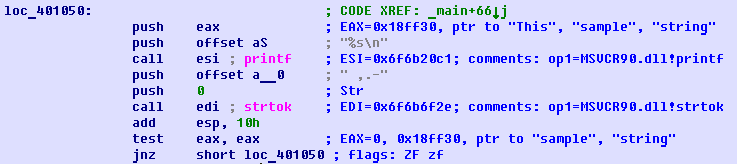
\includegraphics[scale=0.66]{trace_test1.png}
\caption{trace\_test1.png}
\end{figure}

\IFRU{Замечание: "a" это слишком короткая строка для автоматического детектора строк в tracer, поэтому её здесь нет, вместо нее адрес этой строки.}{Note: "a" is too short string for automatic string detector in tracer, that is why it is absent and its address here instead.}

\subsection{\IFRU{Трассируем quicksort()}{Let's trace quicksort()}}

\IFRU{Возьмем известный пример:}{Use well-known example:}

\begin{lstlisting}
//http://cplus.about.com/od/learningc/ss/pointers2_8.htm

/* ex3 Sorting ints with qsort */
//

#include <stdio.h>
#include <stdlib.h>

int comp(const int * a,const int * b) 
{
  if (*a==*b)
    return 0;
  else
    if (*a < *b)
        return -1;
     else
      return 1;
}

int main(int argc, char* argv[])
{
   int numbers[10]={1892,45,200,-98,4087,5,-12345,1087,88,-100000};
   int i;

  /* Sort the array */
  qsort(numbers,10,sizeof(int),comp);
  for (i=0;i<9;i++)
    printf("Number = %d\n",numbers[ i ]);
  return 0;
}
\end{lstlisting}

\IFRU{Трассируем функцию comp():}{Let's trace comp() function:}

\begin{lstlisting}
tracer.exe -l:trace_test2.exe bpf=0x00401030,trace:cc
\end{lstlisting}

\IFRU{Получим после исполнения скрипта в IDA:}{We will get after .idc script execution in IDA:}

\begin{figure}[ht!]
\centering
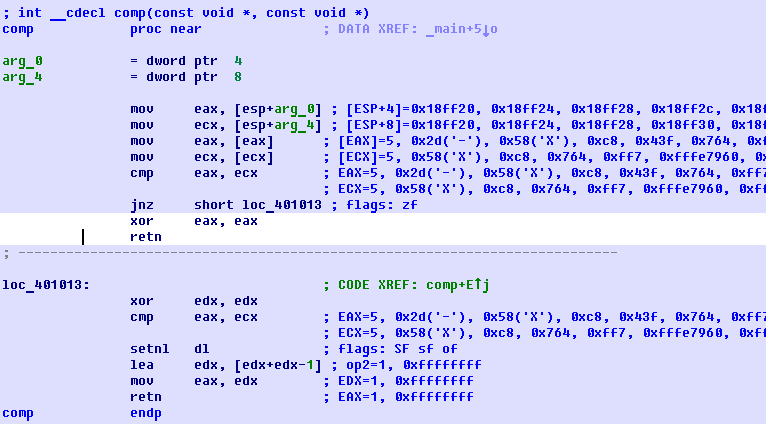
\includegraphics[scale=0.66]{trace_test2.png}
\caption{trace\_test2.png}
\end{figure}

\IFRU{В примере все значения уникальны, одинаковых нет. Таким образом, нет ситуации когда comp() возвращает ноль. Поэтому здесь мы видим что часть comp() возвращающая ноль (xor eax,eax / retn) не была исполнена ни разу.}{In this example all values are unique, there are no equal ones. Therefore, there are no situation when comp() function returning zero. That is why we see that the comp() part returning zero (xor eax,eax / retn) was not executed.}

